\lhead{\begin{tikzpicture}[remember picture, overlay]
    \node [anchor=100,inner sep=0] (imagenIZQUIERDA) at (current page header area.north){
\includegraphics[width=18cm]{img/Encabezado.PNG}};
    \end{tikzpicture}}
    \rhead{Ángeles-Hurtado}
    \rfoot{\begin{tikzpicture}[remember picture, overlay]
    \node [anchor=140,inner sep=0] (imagenDERECHA) at (current page footer area.south){
\includegraphics[width=18cm]{img/Foot.PNG}};
    \end{tikzpicture}}
    %----------------------------------------------------------------------------------------
    \lfoot{ \thepage}
    % \renewcommand{\labelenumi}{\alph{enumi}.)} 
    %----------------------------------------------------------------------------------------
    %----------------------------------------------------------------------------------------
    %	TITLE SECTION
    %----------------------------------------------------------------------------------------
    
    \setlength{\droptitle}{-5\baselineskip} % Move the title up
    \title{\textbf{Estudio de tiempos y movimientos en el ensamble de un circuito electrónico utilizando diferentes métodos para su optimización }} % Article title
    
     \author{ 
         \textsc{Vázquez-Montes,Mitzi Daniela}\\ 
        %  Afiliación:
         \texttt{Instituto Tecnológico de Querétaro} \\ 
         \texttt{Tecnológico Nacional de México} \\ 
         \texttt{Querétaro, México}\\ 
         \texttt{mitzi.vamo25@gmail.com}
     \and 
     \textsc{Ángeles-Hurtado, Luis Alberto}\\ 
    %  Afiliación:
     \texttt{ Instituto Tecnológico de Querétaro } \\ 
     \texttt{ Tecnológico Nacional de México } \\ 
     \texttt{Querétaro, México}\\ 
     \texttt{alb3rt0.ah@gmail.com} 
    }
    
    
    %----------------------------------------------------------------------------------------
    
    % \begin{document}
    
    % Print the title
    \maketitle
    \thispagestyle{fancy}
    
    %----------------------------------------------------------------------------------------
    %	ARTICLE CONTENTS
    %----------------------------------------------------------------------------------------
    
    % \section*{Resumen}
    % \textit{Palabras clave:}
    % El resumen (ancho de página) deberá contener entre 100 y 200 palabras tipo Adobe Devangari 11 puntos.
    
    \begin{abstract}
    \noindent 
    El resumen (ancho de página) deberá contener entre 100 y 200 palabras tipo Adobe Devangari 11 puntos.
    
    \end{abstract}
    % 
    % 
    \textbf{\textit{Palabras clave}}:
    Tiempo,Movimiento
          
    
    \section{Introducción}
    %\begin{itemize}
    El Estudio de Tiempos y Movimientos Se erige como una técnica esencial en la administración de la eficiencia empresarial, fusionando el análisis del tiempo por Frederick Winslow Taylor y el estudio de movimientos por los esposos Frank y Lillian Gilbreth. Esta aproximación, que emplea una diversidad de metodologías, tiene como objetivo primordial mejorar la eficiencia en los procesos industriales y la optimización continua constituye un pilar fundamental en la industria, estas metodologías, entre las cuales se destaca el estudio de tiempos y movimientos, resultan cruciales para comprender y perfeccionar los procesos de fabricación, en este caso el ensamble de un circuito eléctrico utilizando un Protoboard como pieza principal para ensamblar los demás materiales que conforman este circuito. Este análisis permite identificar áreas de mejora y aplicar las metodologías adecuadas para optimizar el proceso de ensamblaje.
    %\end{itemize}
    
    \begin{itemize}
    \item \textbf{{Estudio de tiempos y movimientos}} es el análisis de método, materiales, herramientas e instalación utilizada o que se ha de utilizar en la ejecución de un trabajo. \cite{RAE}
    \item \textbf{Ensamble} es Unir, juntar, ajustar, montar, encajar piezas en pocas palabras es la colocación de dos o más piezas para la conformación de un producto final. \cite{RAE}
    \item \textbf {Circuito electrónico}es un conjunto de elementos eléctricos conectados entre sí que permiten generar, transportar y utilizar la energía eléctrica con la finalidad de transformarla en otro tipo de energía. \cite{RAE}
    \item \textbf{Método de tiempos predeterminados} es una mejora, en pocas palabras se refiere a la capacidad de hacer o resolver alguna cosa de la manera más eficiente posible y, en el mejor de los casos, utilizando la menor cantidad de recursos. \cite{RAE}
    \item \textbf{Optimización} es buscar la mejor manera de realizar una actividad. \cite{RAE}
    \end{itemize}
    
    % 
    % 
    \section{Justificación}
    
    % \begin{itemize}
    
    En la actualidad, la demanda global de productos electrónicos sofisticados y eficientes está en aumento, lo que impulsa la necesidad de mejorar la eficiencia y productividad en la cadena de producción mediante la implementación de estudios de tiempos y movimientos. Estos estudios buscan identificar y eliminar desperdicios en el proceso de ensamblaje, optimizando el uso de tiempo, recursos y energía para maximizar la eficacia.
    A nivel local y nacional, hay una creciente preocupación por el impacto ambiental del ensamblaje de circuitos electrónicos. Los gobiernos pueden promover la adopción de prácticas más sostenibles, incluidos los estudios de tiempos y movimientos, como parte de una estrategia de desarrollo sostenible. Esto podría incluir programas de subsidios para empresas que implementen prácticas más amigables con el medio ambiente.
    
    % \end{itemize}
    % 
    % 
    \section{Descripción del problema}
    \begin{itemize}
        \item Se debe describir la desviación o diferencia del ``es'' con respecto al ``debe ser''.
        \item Se debe hacer alusión a la incógnita científica*.
        \item Debe de tener Referencias científicas, URL, tesis, etc.
    \end{itemize}
    
    \textbf{*La incógnita científica es el elemento cuya solución incrementa el conocimiento científico.}
    % 
    % 
    \section{Fundamentación teórica}
    
    Es la parte medular y de mayor discusión, deberá ser la fundamentación de la hipótesis, por tanto se deberá señalar claramente la razón de la suposición y fundamentación de la misma. Únicamente referencias científicas.
    \begin{itemize}
        \item Se debe de retomar el tema que se planteo en la introducción, pero ahora profundizando para clarificar la incógnita científica y se pueda plantear la hipótesis.
        \item Se debe de retomar la descripción del problema, pero ahora a profundidad del (los) objeto(s) de estudio. 
        \item Se debe de profundizar en las metodologías que se ha usado para el estudio del tema.
        \item Referencias solo de artículos y libros científicos.
    \end{itemize}
    % 
    % 
    \section{Hipótesis}
    
    Es la suposición con fundamento científico relativa a la solución del problema, necesidad o de cómo se aprovecha la oportunidad con la incógnita científica y se fundamenta con: 1. Una suposición (en afirmativo o negativo) y ésta deberá vincularse con:
    2. La fundamentación científica que deberá ser precisa 3. Una entidad de comparación para probar la suposición y
    4. La variable con que se califica o cuantifica la comparación o se prueba la hipótesis.
    
    \begin{itemize}
     \item Se debe de identificar claramente la suposición científica
    \item Se debe de identificar claramente el fundamento científico
    \item Se debe identificar claramente la variable de respuesta
    \item Se debe identifican claramente las realidades o modelos contrastantes
    \item Se debe de establecer las variables asociadas, explicativas o que tienen relación funcional con la variable de respuesta
    \end{itemize}
    % 
    % 
    \section{Objetivo}
    
    \begin{itemize}
        \item Diseña, mejora e integra sistemas productivos de bienes y servicios aplicando tecnologías para su optimización.
        \item Diseña, implementa mejoras de trabajo para elevar la productividad.
    \end{itemize}
    
    \subsection{Objetivos específicos }
    
    En el ensamble del circuito eléctrico, es esencial calcular tanto la media como la varianza, ambas desconocidas. Estas medidas estadísticas son cruciales para comprender y mejorar el proceso de ensamblaje Al analizar estos datos estadísticos, podemos identificar posibles problemas en el proceso de ensamblaje, mejorar la calidad del producto final y así como también encontrar la forma más económica de hacer el trabajo de la producción en la fabricación de circuitos eléctricos.
    La implementación del sistema de tiempos predeterminados generará datos históricos que servirán como punto de referencia para evaluar la productividad. Estos registros históricos proporcionarán información detallada sobre el tiempo requerido para realizar cada tarea en el proceso de ensamblaje. Al utilizar esta información como base de comparación, será posible identificar oportunidades de mejora, optimizar la eficiencia del ensamblaje y establecer estándares realistas para aumentar la productividad en la fabricación de circuitos eléctricos."
    % 
    \section{Cuerpo (Metodología, modelo matemático, etc.)}
    
    \textbf{Metodología para la planificación, diseño y ensamble del circuito electrónico ESP32-C6, con el objetivo de calcular la media y varianza desconocida para generar datos históricos:}
    
    El diseño del circuito es Crear ayudas visuales para el operador que sean claras para su comprensión.
    Preparación de materiales es Verificar que todos los componentes necesarios estén disponibles y en buenas condiciones para su uso.
    \ref{fig:enter-label1}
    
    Preparación del Espacio de Trabajo debes de asegurar un espacio limpio y bien iluminado con herramientas específicas como la almohadilla para soldar, multicontacto, etc.\ref{fig:enter-label2} 
    
    Ensamble de Componentes debes seguir el Manual de ensamblaje del ESP32-C6 para instalar correctamente los componentes.\ref{fig:enter-label3}
    
    Debes de hacer pruebas de manera exhaustiva para así garantizar el funcionamiento correcto, corrigiendo errores si es necesario.
    Documentar y analizar el tiempo dedicado a cada etapa para identificar áreas de mejora.
    
    Una metodología adecuada es crucial para el ensamblaje del circuito ESP32-C6, garantizando eficiencia y precisión. Desde el diseño hasta la documentación y análisis, cada paso es esencial para resultados óptimos. El uso del Método del Tiempo Medido (MTM) permite una evaluación precisa y mejora continua. Esto facilita la obtención de datos históricos y proporciona una base sólida para optimizar procesos futuros.
    \begin{figure}[H]
        \centering
        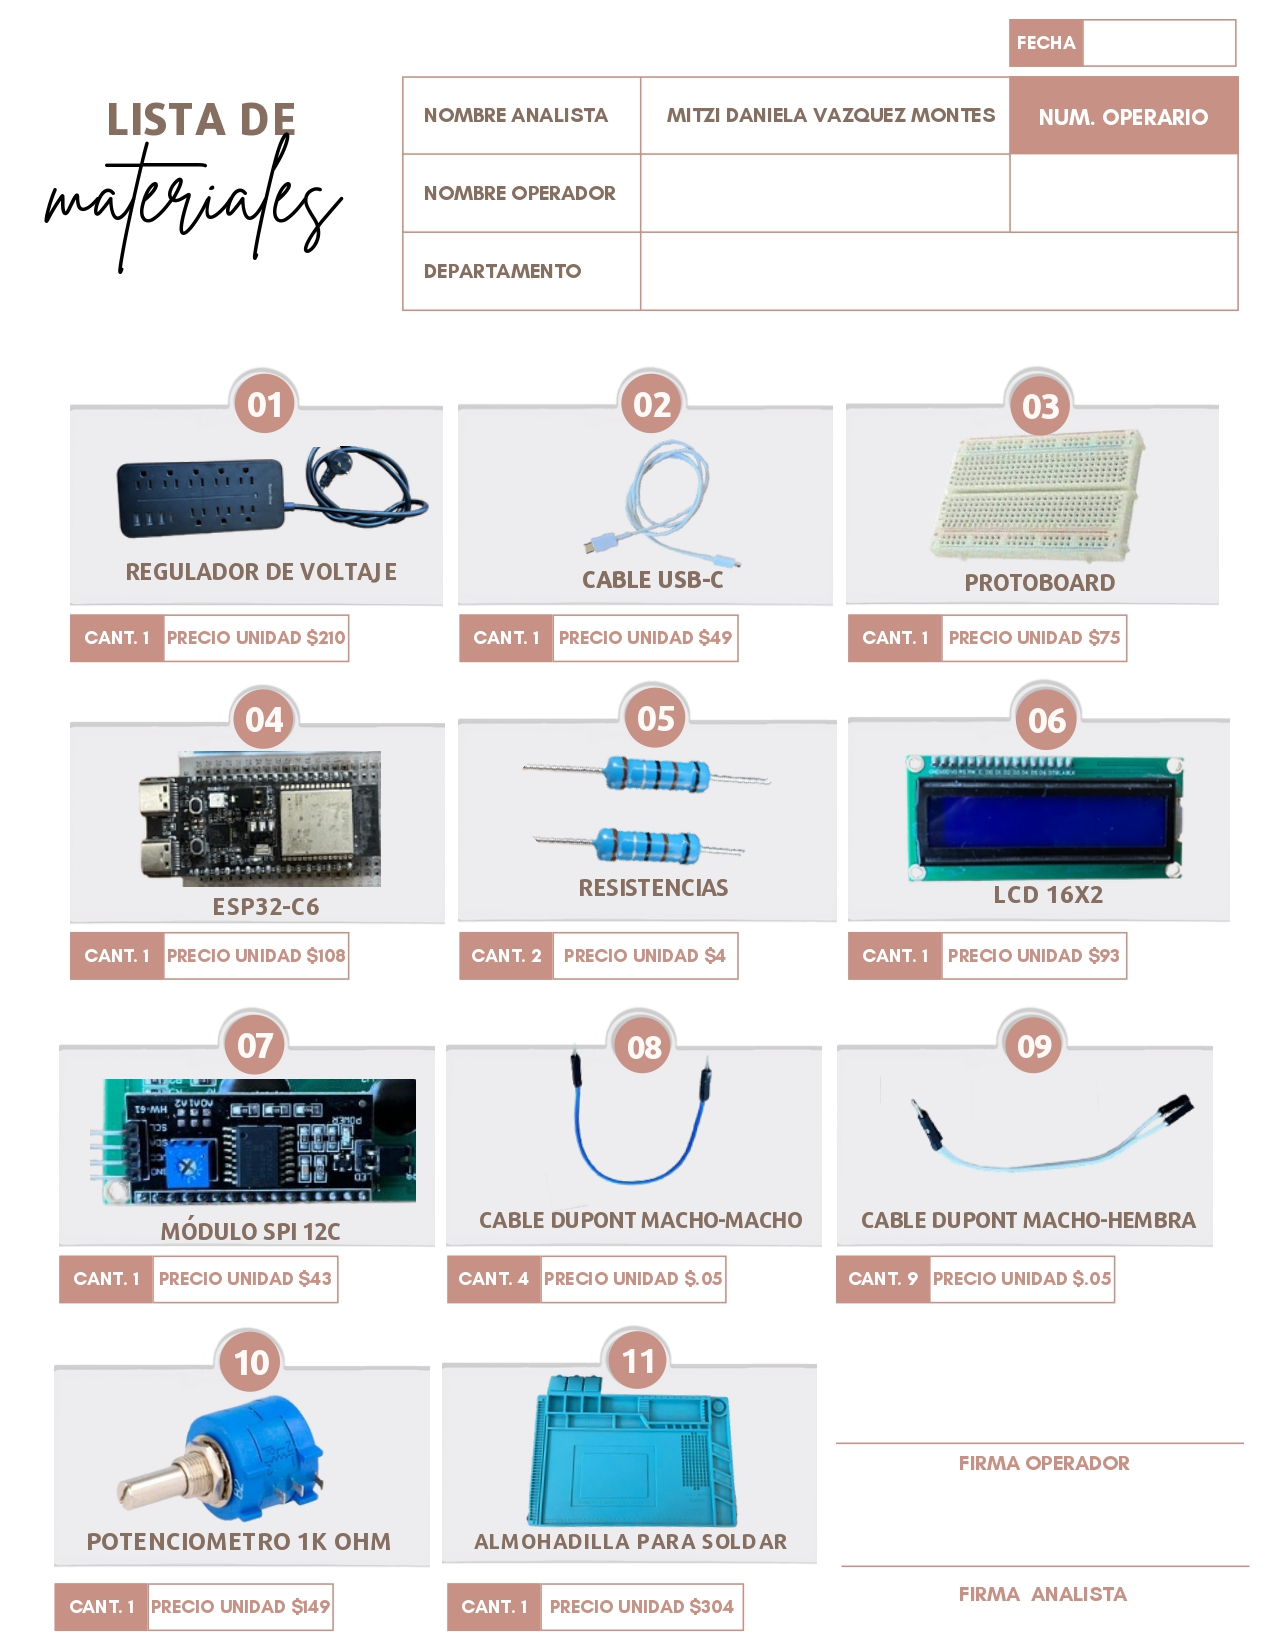
\includegraphics[trim = {1mm 1mm 1mm 1mm},clip,scale=0.2]{34/img/listaMateriales.png}
        \caption{Lista de materiales}
        \label{fig:enter-label1}
    \end{figure}
    \begin{figure}[H]
        \centering
        \includegraphics[trim = {1mm 1mm 1mm 1mm},clip,scale=0.2]{34/img/bosquejo.png}
        \caption{Bosquejo}
        \label{fig:enter-label2}
    \end{figure}
    \begin{figure}[H]
        \centering
        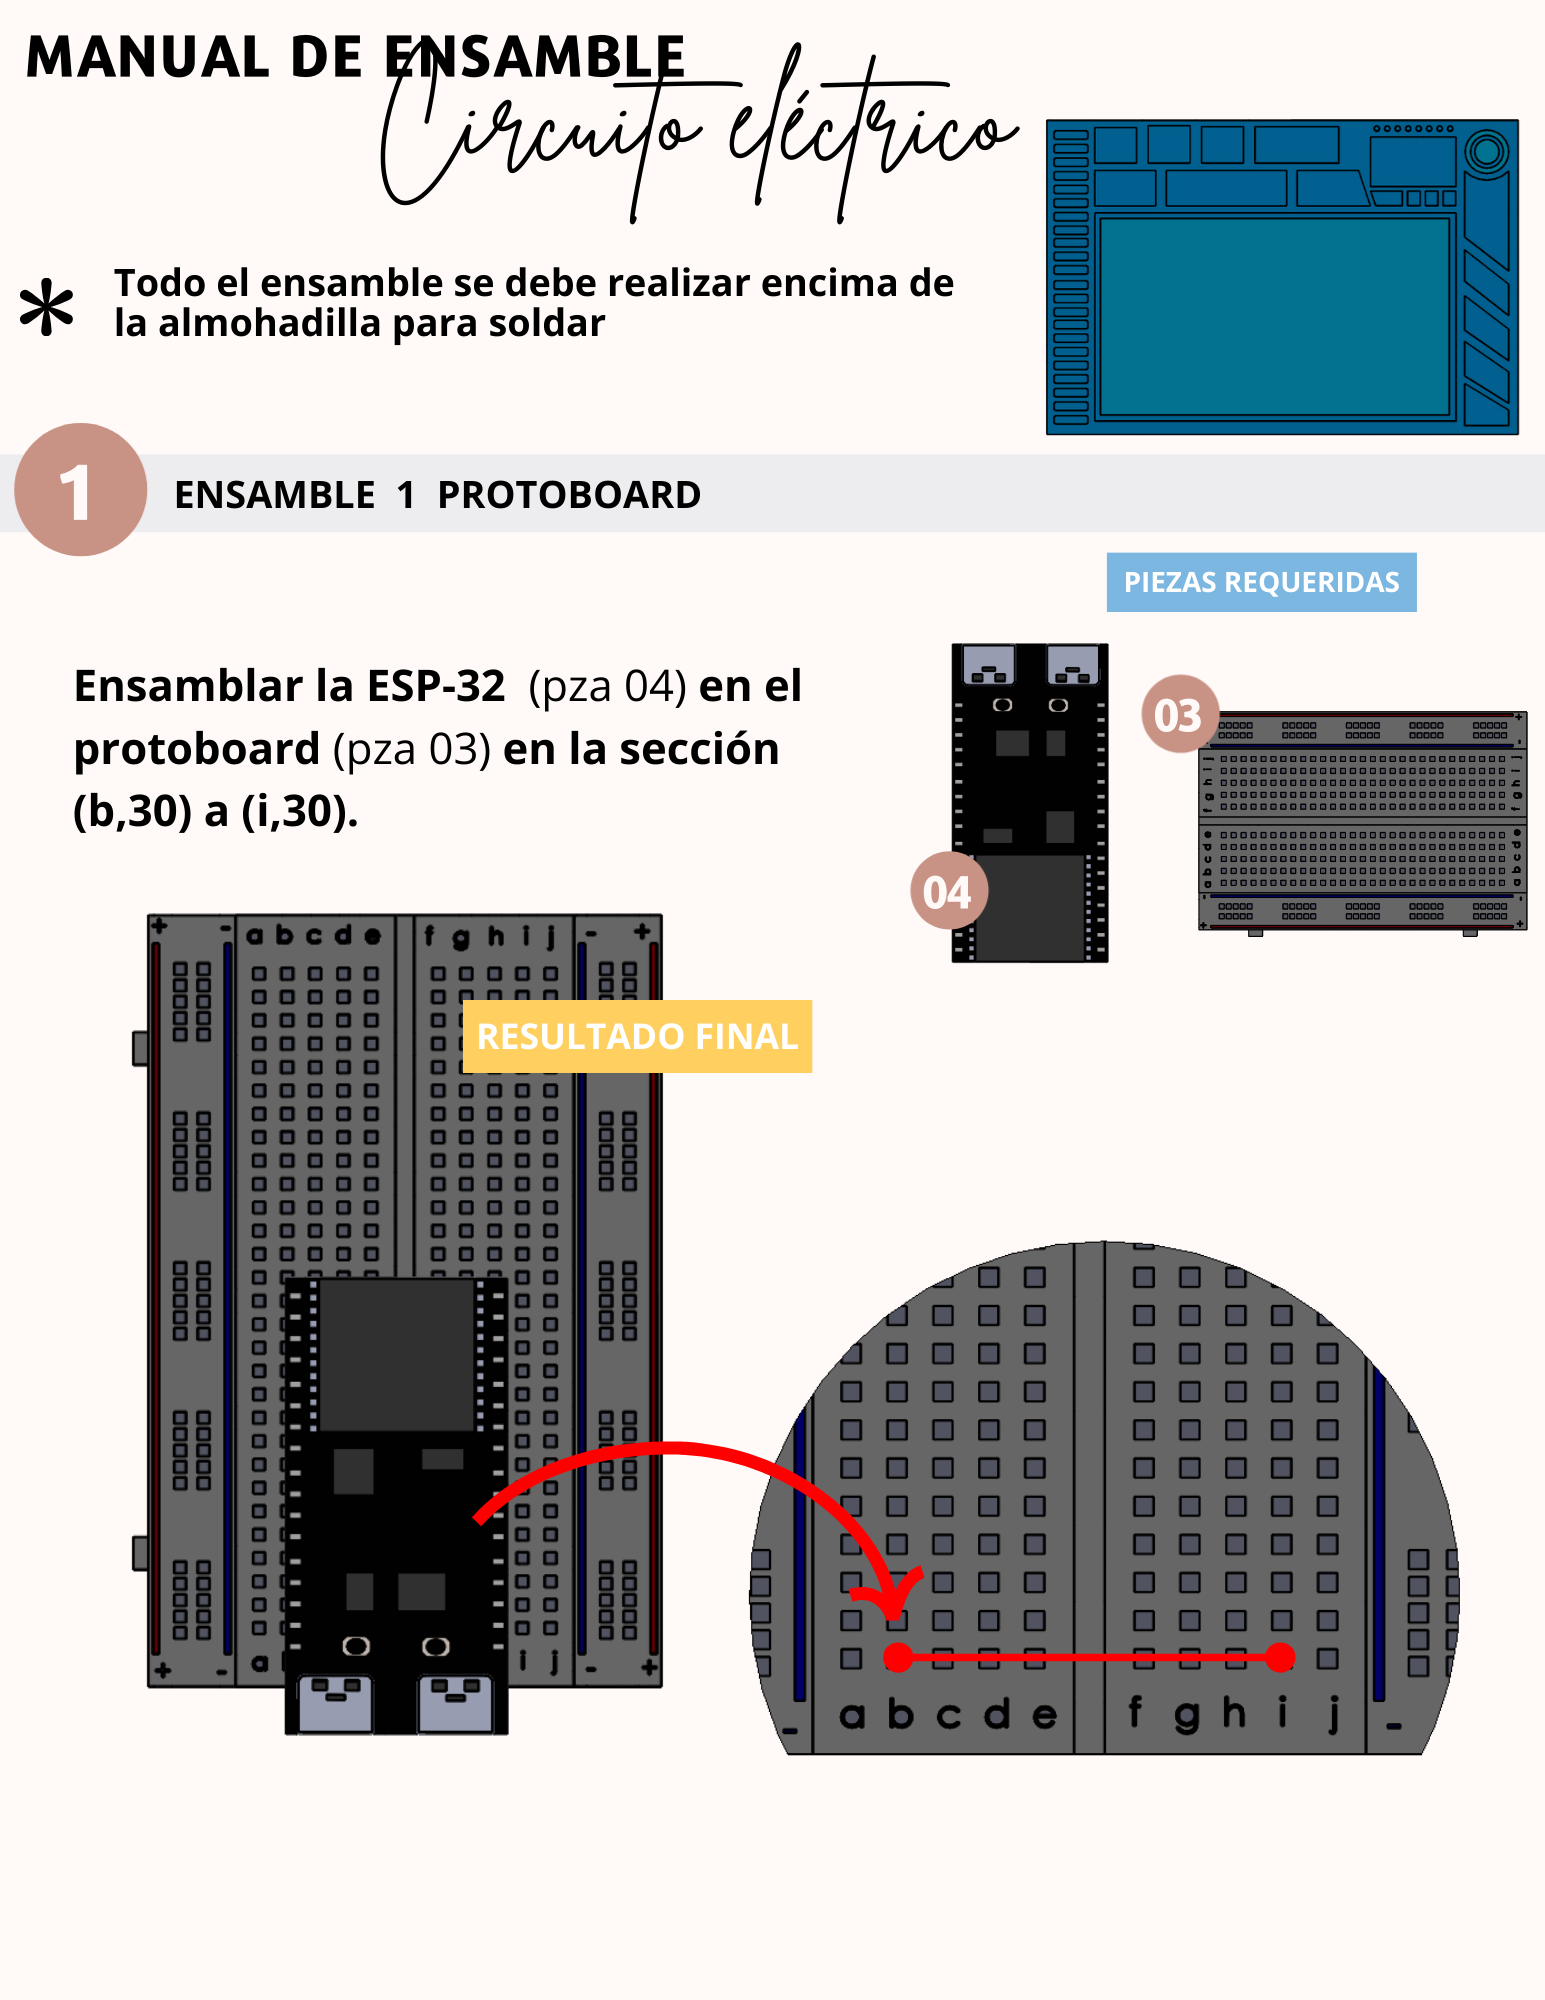
\includegraphics[trim = {1mm 1mm 1mm 1mm},clip,scale=0.2]{34/img/pasosEnsamble.png}
        \caption{Pasos ensamble}
        \label{fig:enter-label3}
    \end{figure}
    % 
    % 
    % \begin{figure}[H]
    %     \centering
    %     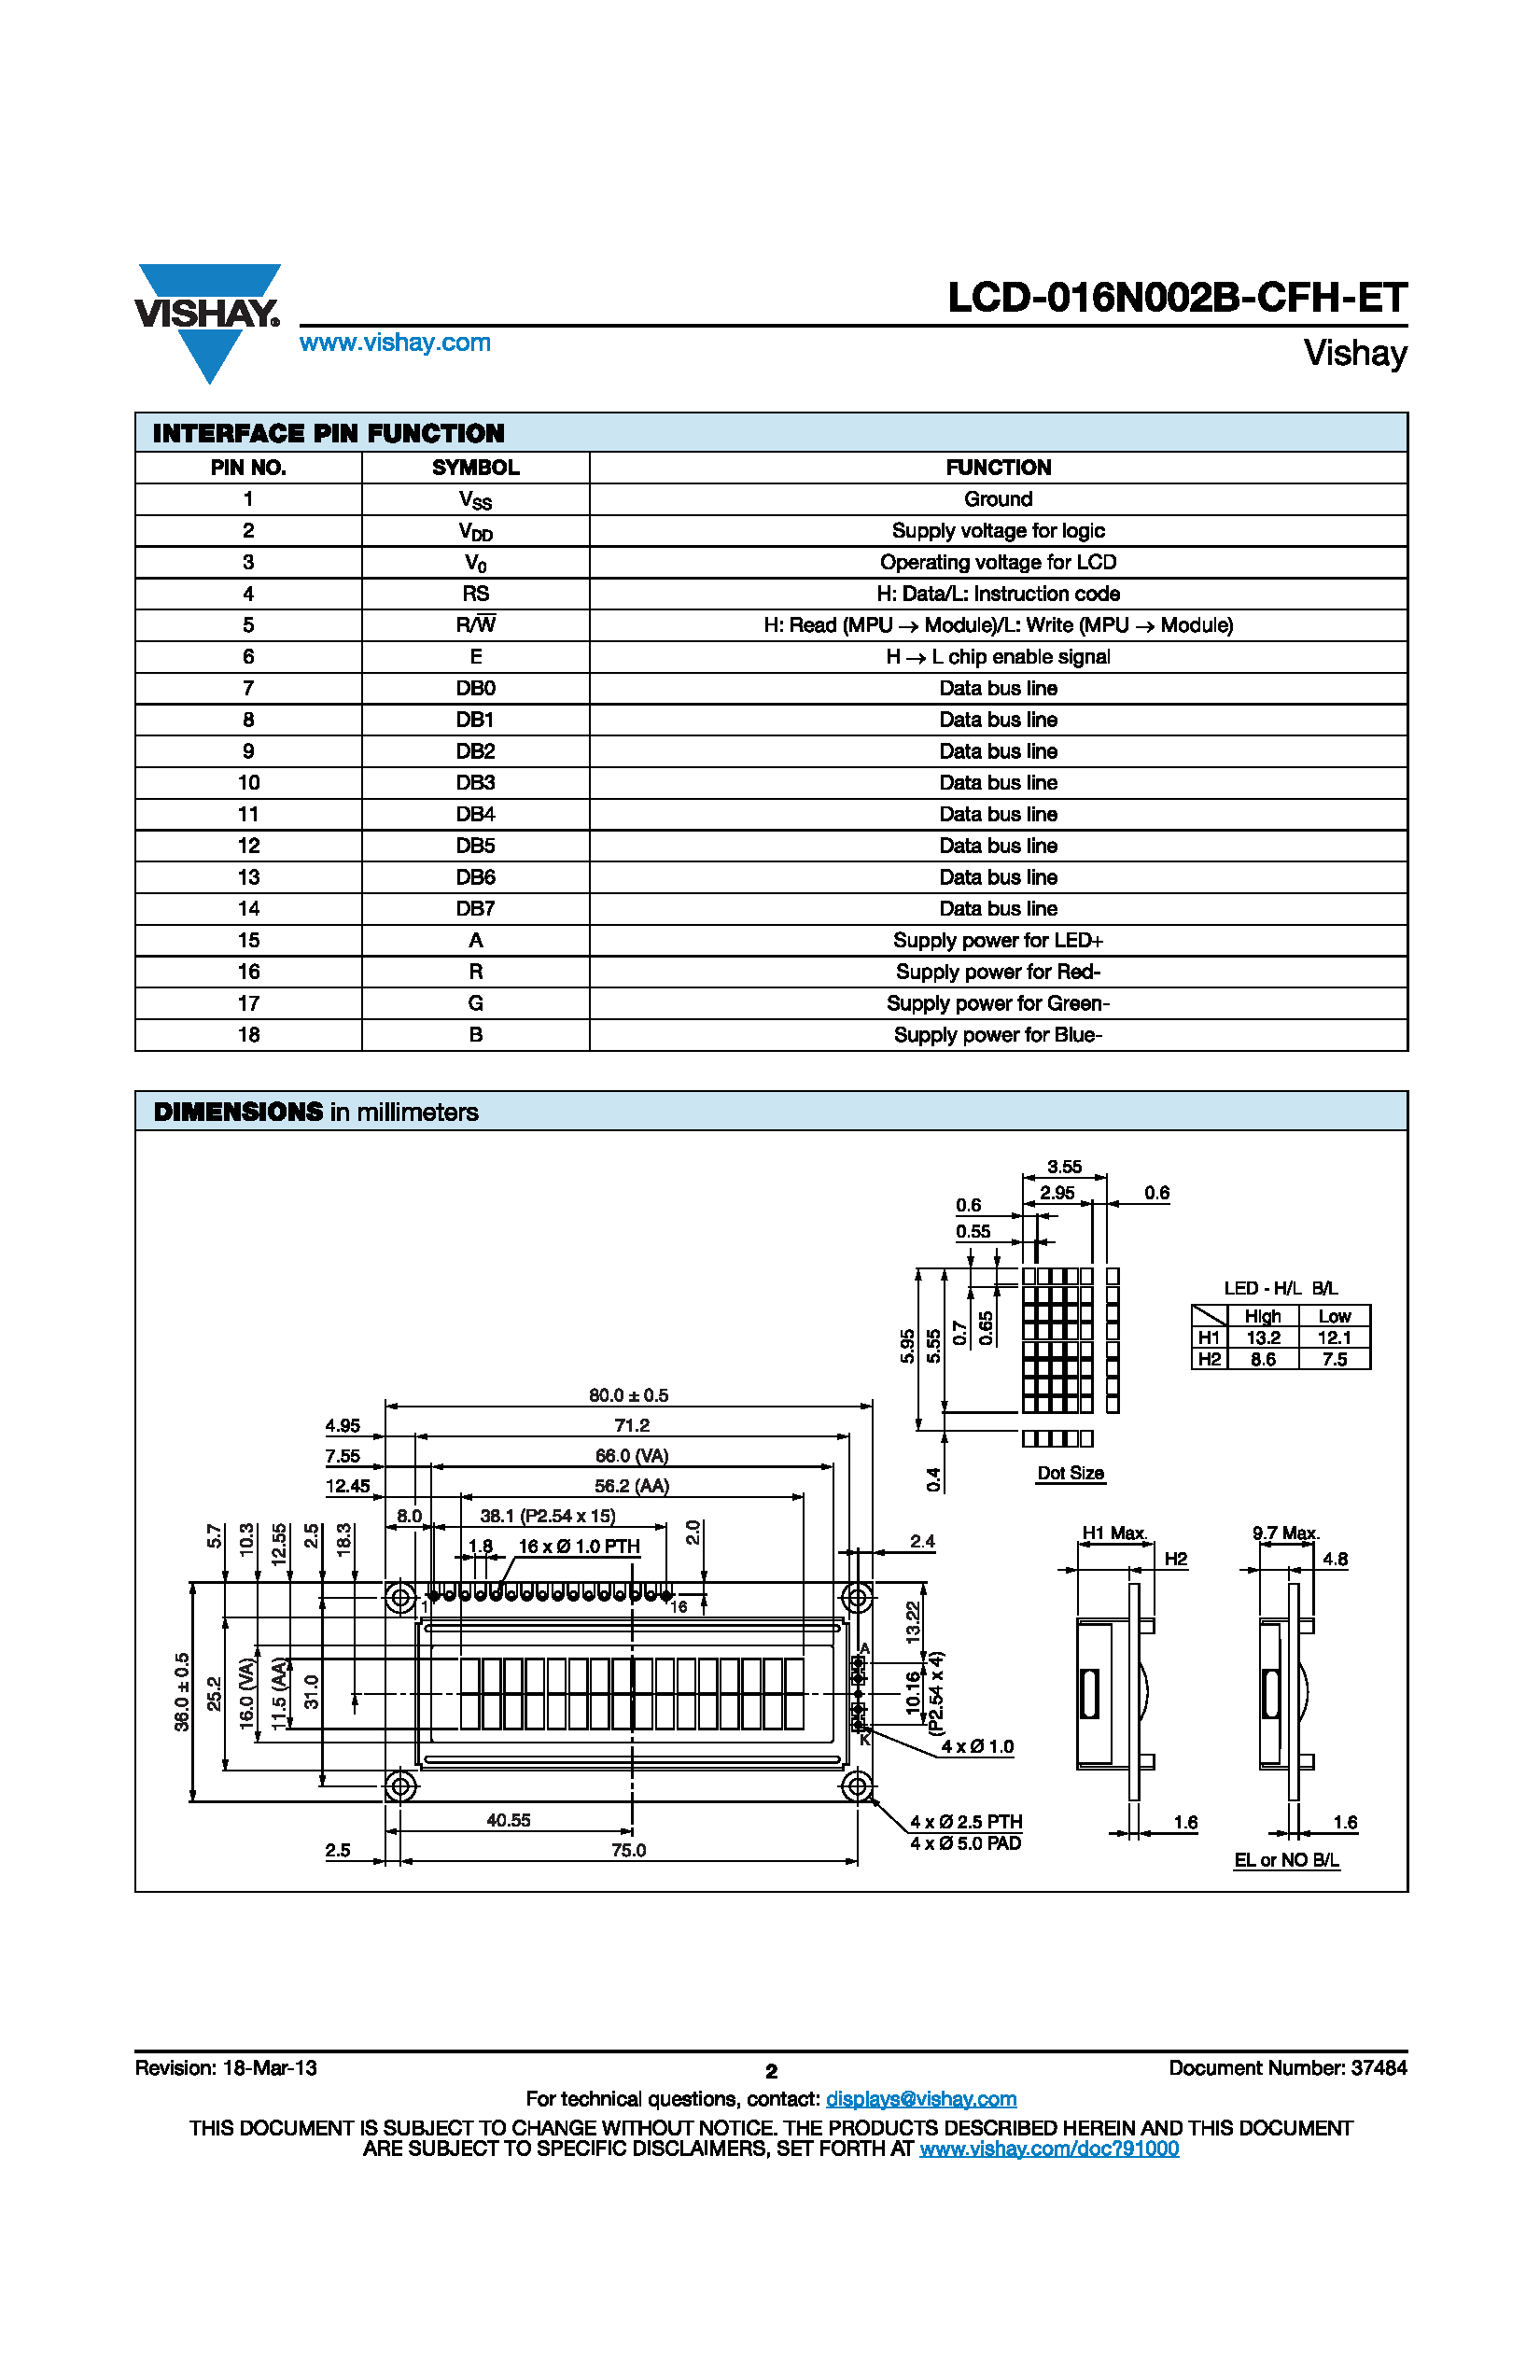
\includegraphics[trim = {30mm 250mm 90mm 20mm},clip,scale=0.5]{6/Img/lcd-16x2.pdf}
    %     \caption{Esquema LCD de 16x2}
    %     \label{fig:lcd-16x2}
    % \end{figure}
    % 
    % 
    \subsection{Acrónimos y Abreviaciones}
    
    Los acrónimos y abreviaciones deberán ser definidos únicamente la primera vez que aparecen en el texto, esto para que el lector entienda lo que significan.
    
    \subsection{Ecuaciones}
    
    Las ecuaciones son una excepción a las especificaciones prescritas de esta plantilla. 
    Deberá determinar si su ecuación debe escribirse o no utilizando la fuente Adobe Devangari. 
    Para crear ecuaciones multinivel, puede ser necesario tratar la ecuación como un gráfico e insertarla en el texto después de aplicar el estilo de la platilla.
    Las ecuaciones serán enumeradas de manera consecutiva, y el número de ecuación, entre paréntesis, se colocan al ras de la derecha, utilizando una tabulación derecha. 
    
    \begin{equation}
        \label{eq1}
        x + y = z 
    \end{equation}
    
    Es importante asegurarse de que los símbolos de la ecuación sean definidos antes o inmediatamente después de la ecuación. Utilice “(1)”, en vez de “Eq. 1” al enumerar las ecuaciones, excepto al principio de una oración: “La ecuación (\ref{eq1}) es…”
    
    \section{Resultados y discusión}
    
    Antes de comenzar a preparar tu artículo, es importante que lea primero la guía del autor, la cual incluye los temas o apartados que son necesarios para tener tu trabajo completo.
    Una vez completada la edición del texto, el documento está listo para el uso de esta plantilla. En este archivo recién creado, resalte todo el contenido e importe el archivo de texto preparado. Ahora esta listo para estilizar su documento.
    En esta sección se deben presentar todo lo obtenido de la sección 2, incluidas deducciones o efectos del desarrollo. También se podrán incluir subsecciones numeradas de la siguiente forma:
    
    
    \newpage
    \centering{\section[\appendixautorefname{}]{Apéndice}}\label{anexo:fotosDeEvidencia}
    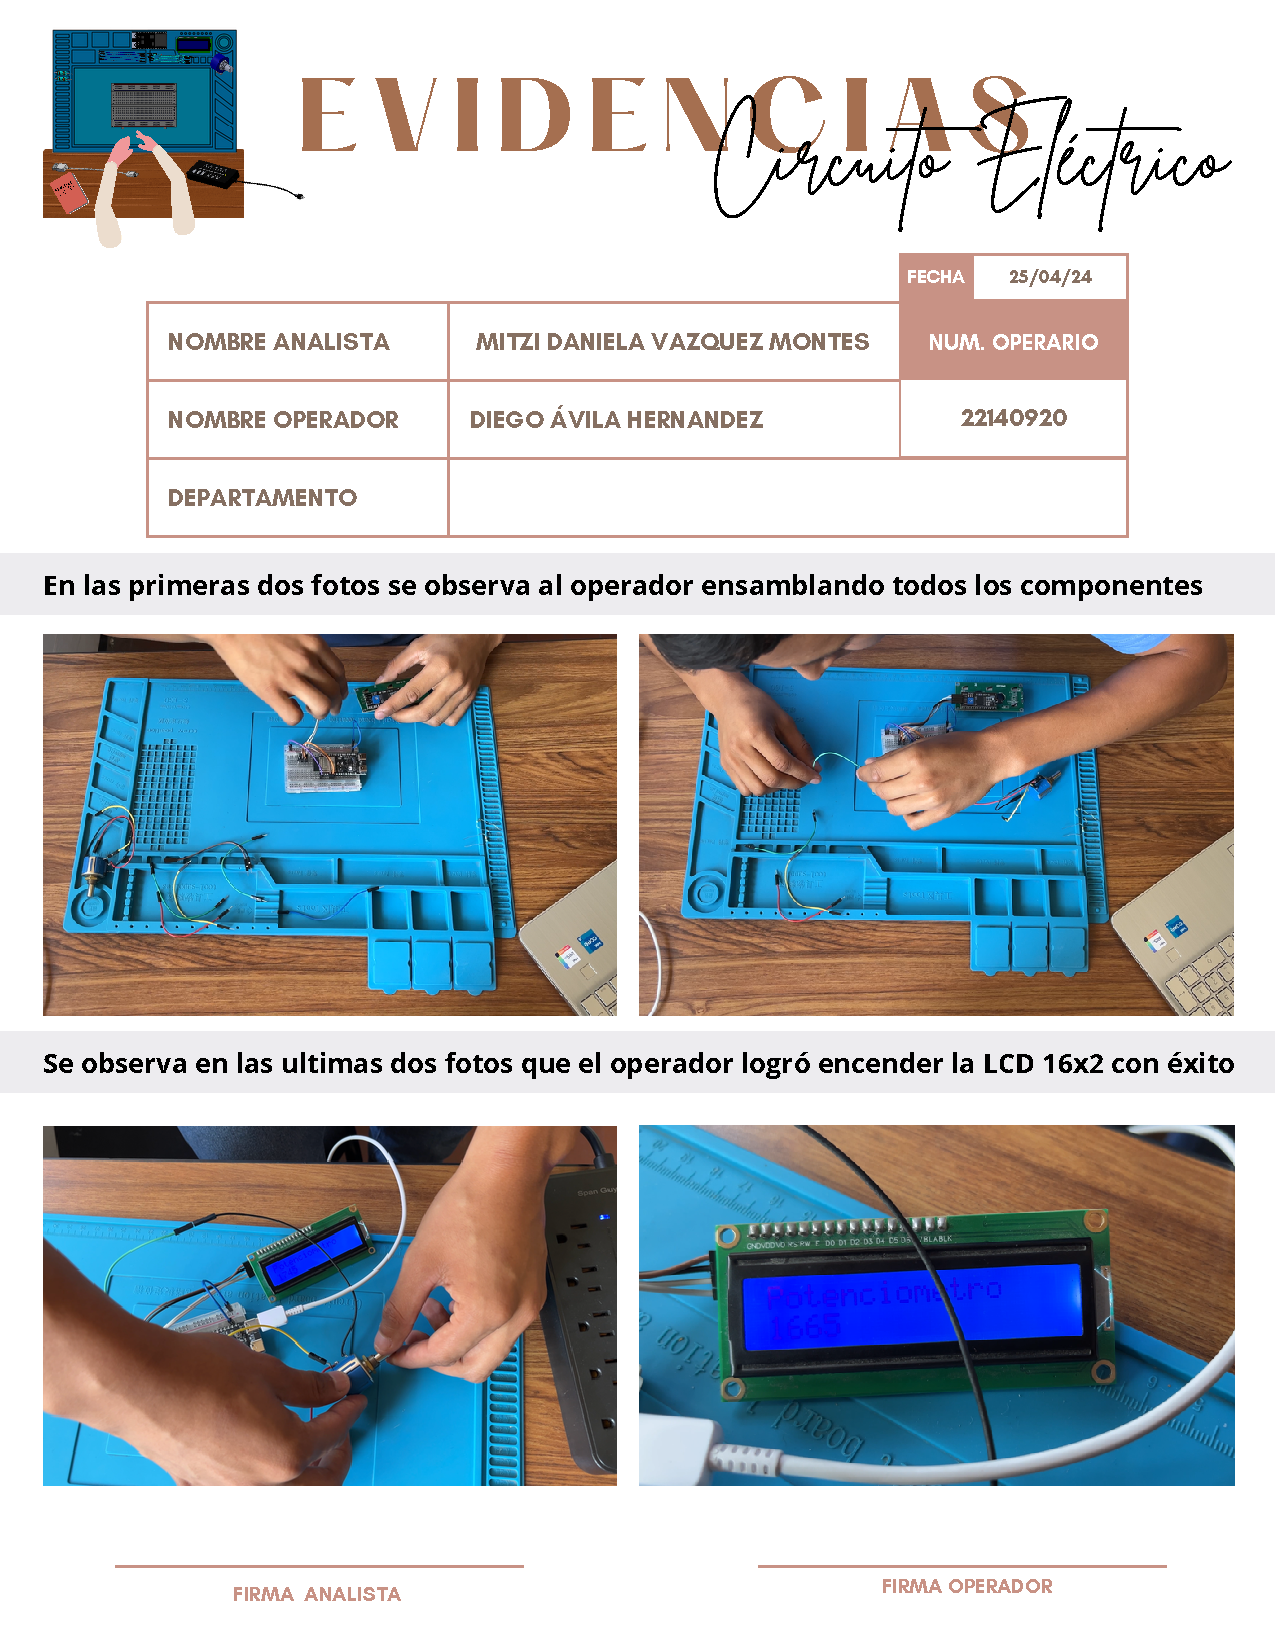
\includepdf[pages=-]{34/img/fotosDeEvidencia.pdf}
    
    \subsection{Autores y Afiliaciones}
    
    Para distinguir las afiliaciones de los autores, utilice superíndices iniciando con el número 1, 2, etc., sucesivamente, esto dependerá de la cantidad de los departamentos a los que estén afiliados los autores. En caso de que todos los autores pertenezcan a una mismo departamento e institución, utilizar sólo el superíndice 1. 
    
    \subsection{Identificar los encabezados}
    
    Se les recuerda a los autores que los encabezados deben de estar conforme los solicita la guía del autor. De ahí se puede adaptar el trabajo para que sea más fácil de entender para el lector.
    Los encabezados organizan los temas sobre una base relacional y jerárquica. Por ejemplo, el título del documento es encabezado del texto principal porque todo el material posterior se relaciona y elabora sobre este tema. 
    
    \subsection{Tablas y Figuras}
    
    \begin{enumerate}
        \item Posición de las tablas y figuras: Coloque las figuras y las tablas en la parte superior e inferior de las columnas. Evite colocarlos en medio. Las figuras y las tablas grandes pueden abarcar ambas columnas. Los títulos de las figuras deben de estar debajo de las mismas; los títulos de las tablas deben aparecer encima de ellas. Insértese las figuras y los cuadros después de citarse en el texto. Utilice la abreviatura “Fig. 1”, incluso al principio de una oración. 
    \end{enumerate}
    
    \section{Conclusiones}
    
    Se describe aquí el alcance del trabajo, logros obtenidos y perspectivas para el futuro de este. Se sugiere colocar información cuantitativa obtenida.
    
    \section{Agradecimientos}
    
    Es importante darles su debido reconocimiento a los laboratorios, instituciones, organizaciones, entre otros que han sido participes para la culminación de este trabajo. También es importante mencionar, fondos, proyectos, becas, entre otros que se le han otorgado al o los autores para realizar el trabajo de investigación. Ejemplo: “Los autores agradecen al Concejo Nacional de Ciencia y Tecnología por los recursos otorgados…”
    
    \section*{Referencias}
    
    %Para esta platilla, se solicita al autor enumerar las citas de manera consecutiva entre corchetes \cite{YLi2013}. 
    %La puntuación de la oración que sigues sería \cite{Mesaelides2011}. 
    %Refiérase simplemente al número de referencia, como en \cite{Morales2012}, no utilice “Ref. [3]” o “referencia [3]” excepto al principio de una oración: “La referencia [3] fue la primera…”
    Enumere las notas al pie por separado en superíndices. Coloque la nota de pie de en la parte inferior de la columna en la que se citó. No coloque notas al pie en la lista de referencias. Utilice letras para las notas al pie de la tabla.
    A menos de que haya tres autores o más; no utilice “et al.”. Los trabajos que no hayan sido publicados, incluso si han sido presentados para su publicación, deben ser citados como “inéditos”. Los trabajos que han sido aceptados para su publicación deben de citarse como “en prensa”. Poner en mayúscula sólo la primera palabra de un título, excepto los nombres propios y los símbolos de elemento. 
    %Otros ejemplos \cite{LAAngeles2021}, \cite{LAAngelesConni}. 
    %Véase el archivo adjunto \ref{anexo:pines}.
    
    % Ejemplo
    %  @Article{article,
    % 	author = "Author1 LastName1 and Author2 LastName2 and Author3 LastName3",
    % 	title = "Article Title",
    % 	volume = "30",
    % 	number = "30",
    % 	pages = "10127-10134",
    % 	year = "2013",
    % 	doi = "10.3389/fnins.2013.12345",
    % 	URL = "http://www.frontiersin.org/Journal/10.3389/fnins.2013.12345/abstract",
    % 	journal = "Frontiers in Neuroscience"
    % }
    
    % @book{book,
    %   author    = {Author Name}, 
    %   title     = {The title of the work},
    %   publisher = {The name of the publisher},
    %   address   = {The city},
    %   year      = 1993,
    % }
    
    % @incollection{chapter,
    %   author       = {Bauthor Surname}, 
    %   title        = {The title of the work},
    %   editor       = {Editor Name},
    %   booktitle    = {The title of the book},
    %   publisher    = {The name of the publisher},
    %   address      = {The city},
    %   year         = 2002,
    %   pages        = {201-213},
    % }
    
    % @InProceedings{conference,
    %   author = {Cauthor Name and Dauthor Surname and Fauthor LastName},
    %   title = {The title of the work},
    %   booktitle = {The title of the conference proceedings},
    %   year = 1996,
    %   publisher = {The name of the publisher},
    %   editor = {Editor Name1 and Editor Name2},
    %   pages = {41-50},
    % }
    
    % @book{cho,
    %   author       = {Gauthor Name1}, 
    %   title        = {The title of the work},
    %   publisher = {Country code and patent number},
    %   address      = {Patent Country},
    %   year = 2013
    % }
    
    % @book{patent,
    %   author    = {Hauthor Surname1}, 
    %   title     = {The title of the work},
    %   publisher = {Patent number},
    %   address   = {Patent country},
    %   year      = 2010,
    % }
    
    % % please use misc for datasets
    % @misc{dataset, 
    % 	author = "Author1 LastName1 and Author2 LastName2 and Author3 LastName3",
    % 	title = "Data Title",
    % 	year = "2011",
    % 	doi = "10.000/55555",
    % 	URL = "http://www.frontiersin.org/",
    % 
     
    \bibliographystyle{ieeetr}
    \bibliography{34/referencias}
    % 
    % 
    %%%%%%%%%%%%%%%%%%%%%%%%%%%%%%%%%%
    \appendix
    %%%%%%%%%%%%%%%%%%%%%%%%%%%%%%%%%%
    % 
    % 
    \centering{\section[\appendixautorefname{}]{Apéndice}}\label{anexo:manual}
    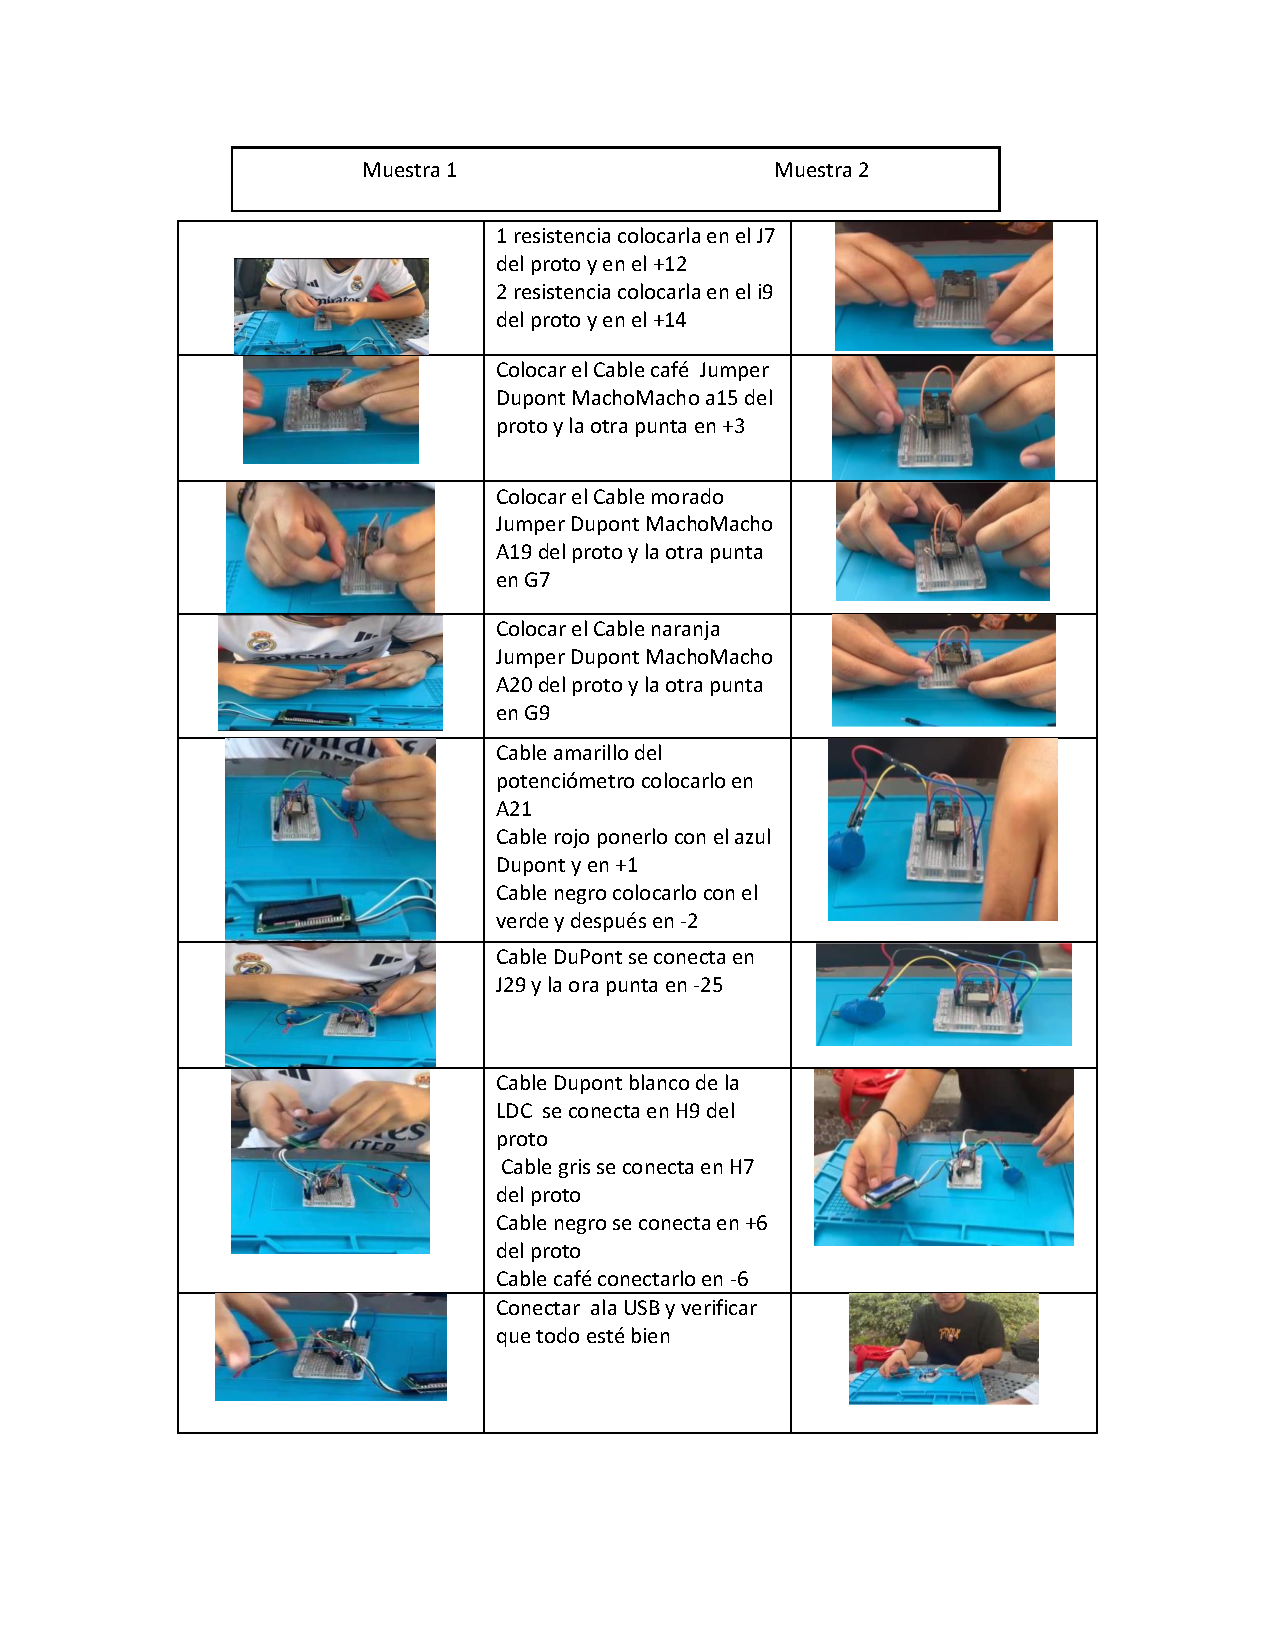
\includepdf[pages=-]{34/img/manual.pdf}
    %%%%%%%%%%%%%%%%%%%%%%%%%%%%%%%%%%%%%%%%